\documentclass[aspectratio=169,usenames,dvipsnames]{beamer}


\usetheme{default}  % You can choose any other theme you prefer

\title{06 - Algoritmos}
\subtitle{Interseção de Segmentos}
\author{Mateus Oliveira de Figueiredo}
\date{19/10/2023}

\usepackage{tikz}
\usetikzlibrary{matrix}
\usepackage{multicol}
\usepackage{algorithm}
\usepackage{algpseudocode}
\usepackage{xcolor}
\usepackage[utf8]{inputenc}
\usepackage[portuguese]{babel}
\usepackage{amsmath} % for "pmatrix" environment  

\usepackage{pgfplots}
\DeclareUnicodeCharacter{2212}{−}
\usepgfplotslibrary{groupplots,dateplot}
\usetikzlibrary{patterns,shapes.arrows, positioning}
\pgfplotsset{compat=newest}

\begin{document}

\begin{frame}
\titlepage
\end{frame}

\begin{frame}
\frametitle{Algoritmos Implementados}
\vfill
\begin{itemize}
  \item Força Bruta ({\it{Naive}})
  \item Algoritmo de Bentley-Ottmann
\end{itemize}
\vfill
\end{frame}

\foreach \n in {0,...,14} {
\begin{frame}
\frametitle{Algoritmo de Bentley-Ottmann - Detecção}
    \begin{figure}
      \includegraphics[width=0.6\textwidth]{figs/event_\n.pdf}
    \end{figure}
\end{frame}

}

\begin{frame}{Estruturas de Dados}
  
  \vfill
  Para guardar os segmentos que estão ativos:
  \begin{itemize}
    \item Lista Ordenada
    \item Lista Não Ordenada
    \item Árvore Binária
    \item Árvore AVL
  \end{itemize}

  \vfill
  Estrutura de eventos no caso de detecção de interseção foi usado uma lista.
  \vfill
\end{frame}

\begin{frame}{Exemplos Randomizados}
  \begin{columns}
    \begin{column}{0.5\textwidth}
      \begin{figure}
        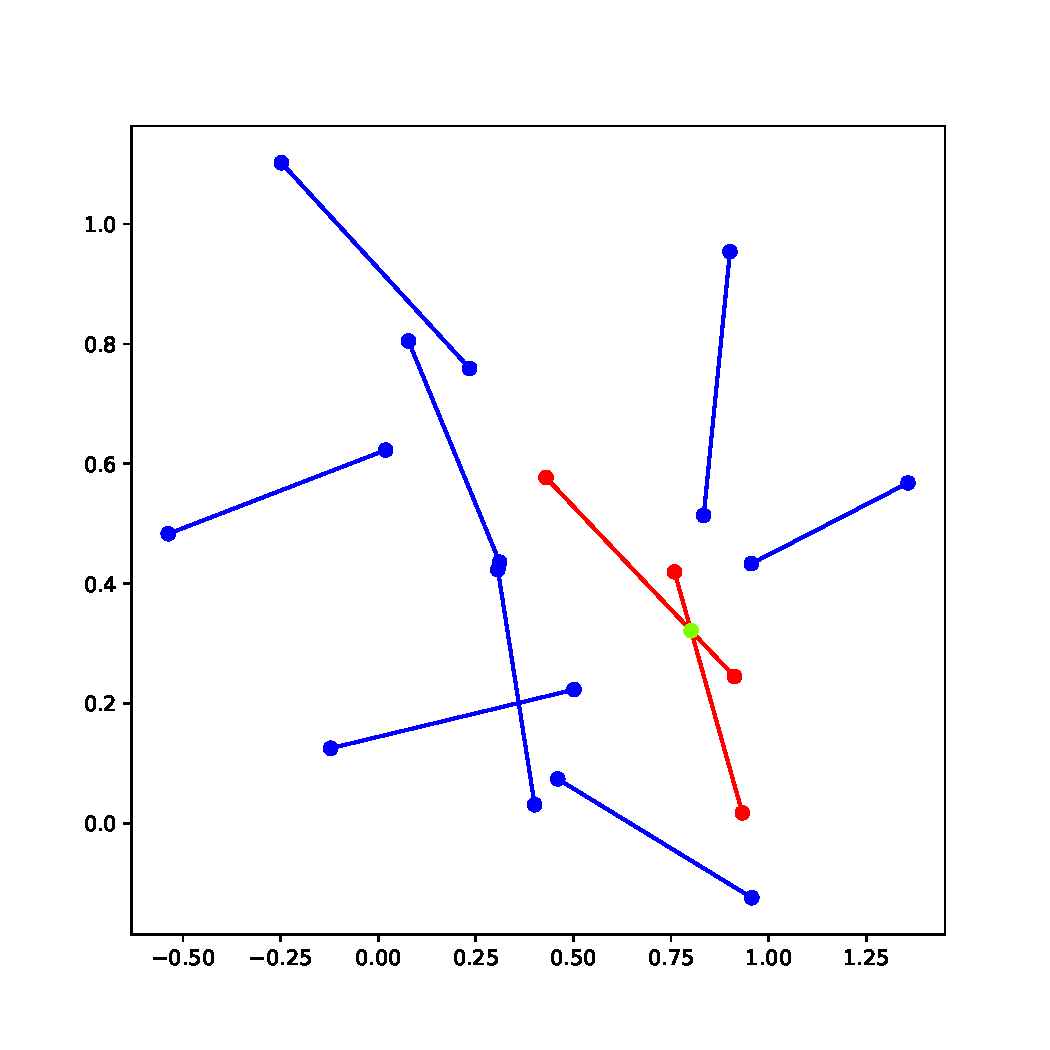
\includegraphics[width=0.9\textwidth]{figs/examples_0.pdf}
        \caption{10 Segmentos Sorteados}
      \end{figure}
    \end{column}
    \begin{column}{0.5\textwidth}
      \begin{figure}
        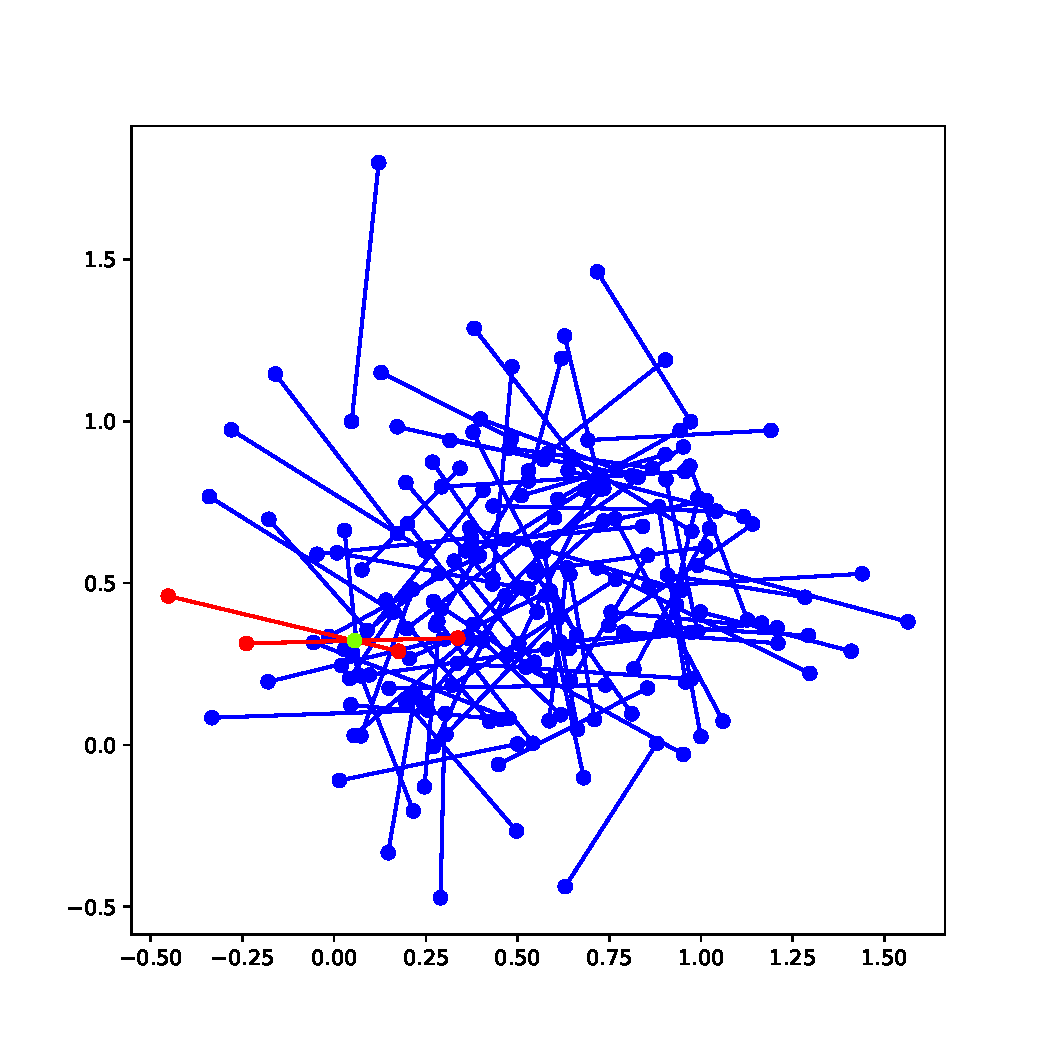
\includegraphics[width=0.9\textwidth]{figs/examples_1.pdf}
        \caption{100 Segmentos Sorteados}
      \end{figure}
    \end{column}
  \end{columns}
\end{frame}

\begin{frame}{Exemplos Sem Interseção - Segmentos Grandes}
  % Two columns
  \begin{columns}
    \begin{column}{0.35\textwidth}
      \begin{figure}
        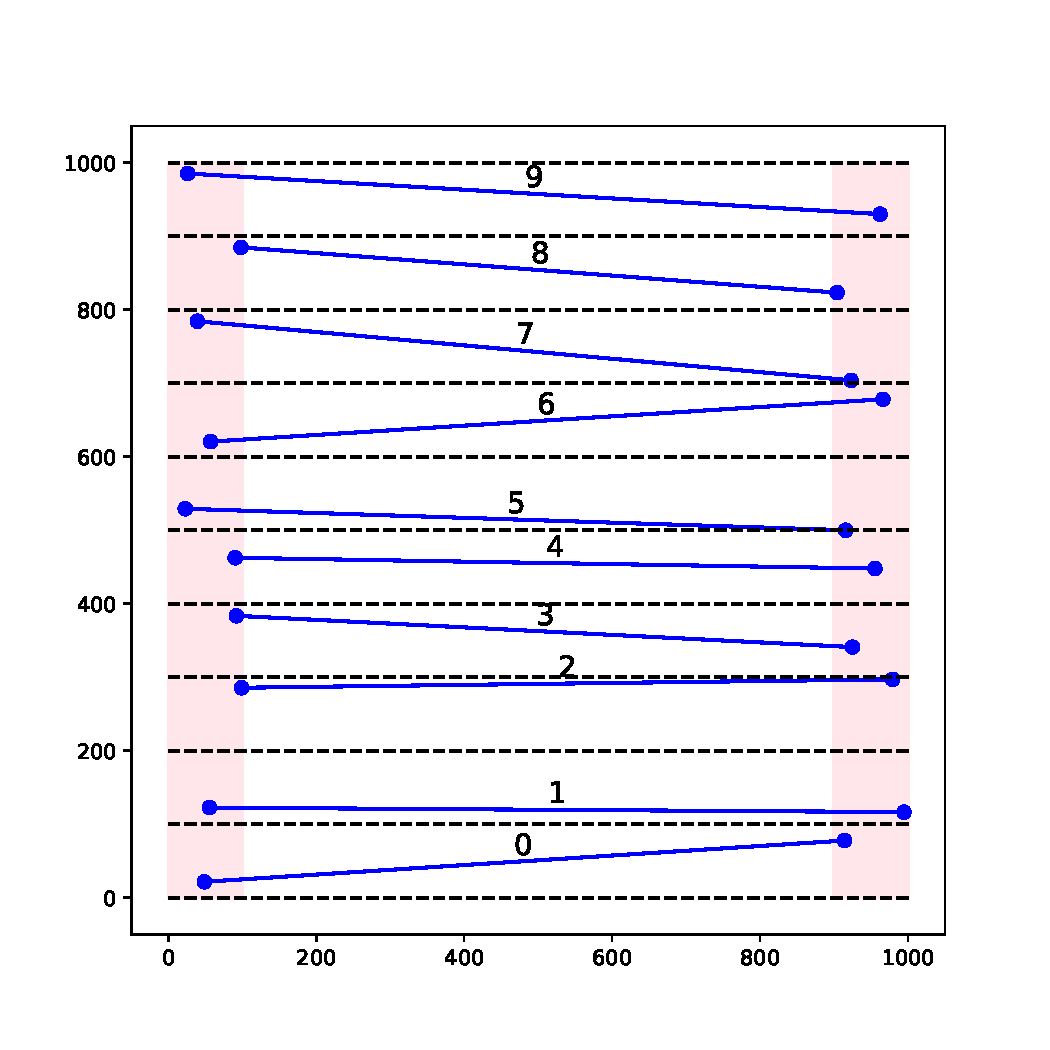
\includegraphics[width=\textwidth]{figs/big_example.pdf}
      \end{figure}
    \end{column}
    \begin{column}{0.65\textwidth}
      \begin{figure}
        \onslide<2>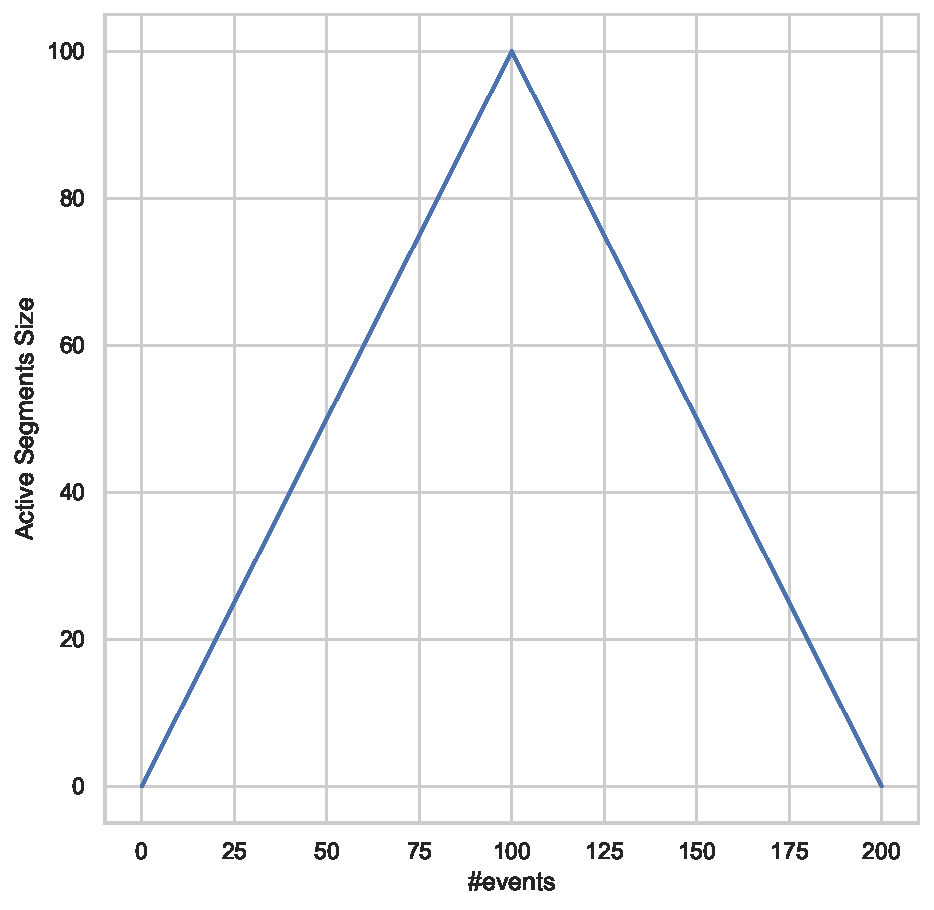
\includegraphics[width=0.9\textwidth]{figs/ativos/big_detection_segments_size_100.pdf}
      \end{figure}
    \end{column}
  \end{columns}
\end{frame}

\begin{frame}{Exemplos Sem Interseção - Segmentos Grandes}
  % Two columns
     \begin{figure}
        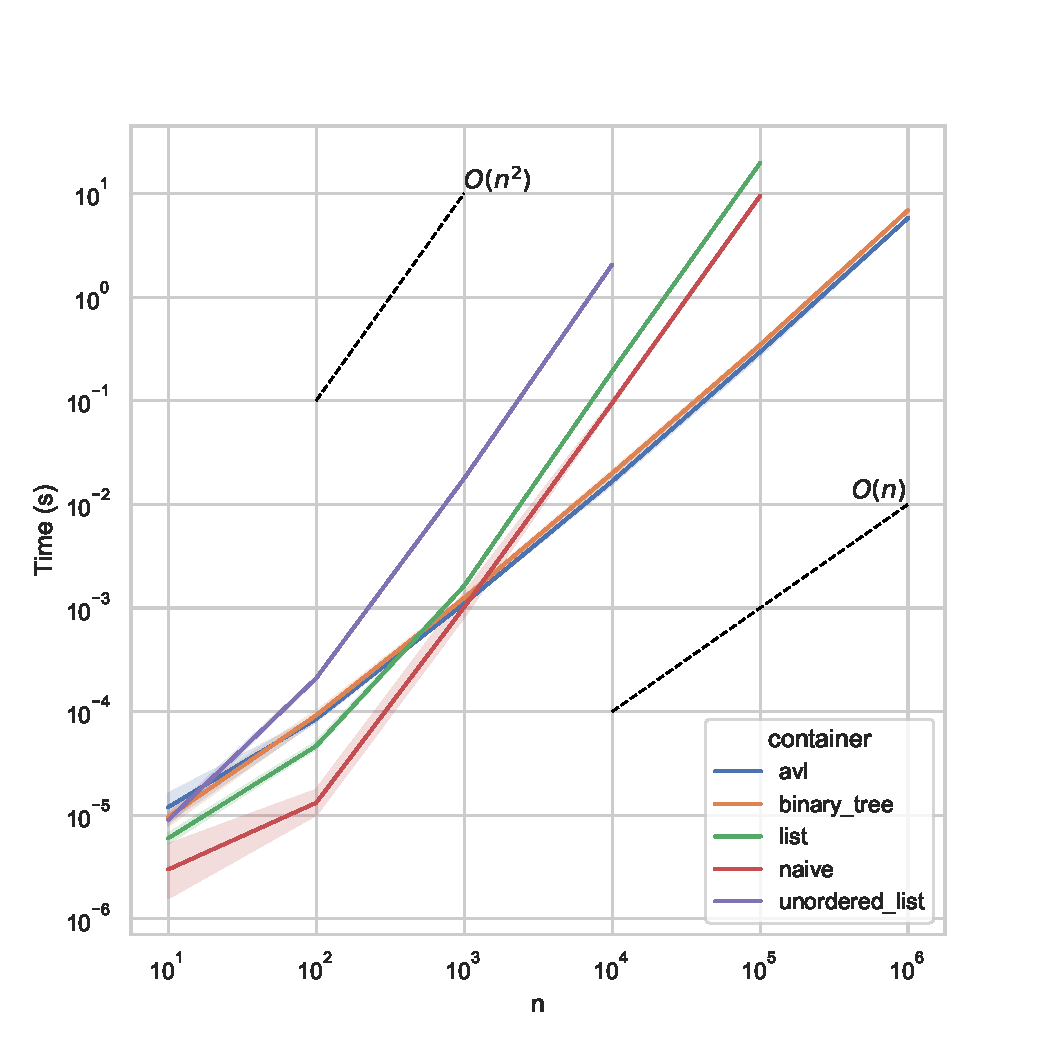
\includegraphics[width=0.5\textwidth]{figs/tempos/plot_big_detection_time.pdf}
      \end{figure}
\end{frame}

\begin{frame}{Exemplos Sem Interseção - Segmentos Pequenos}
  % Two columns
  \begin{columns}
    \begin{column}{0.35\textwidth}
      \begin{figure}
        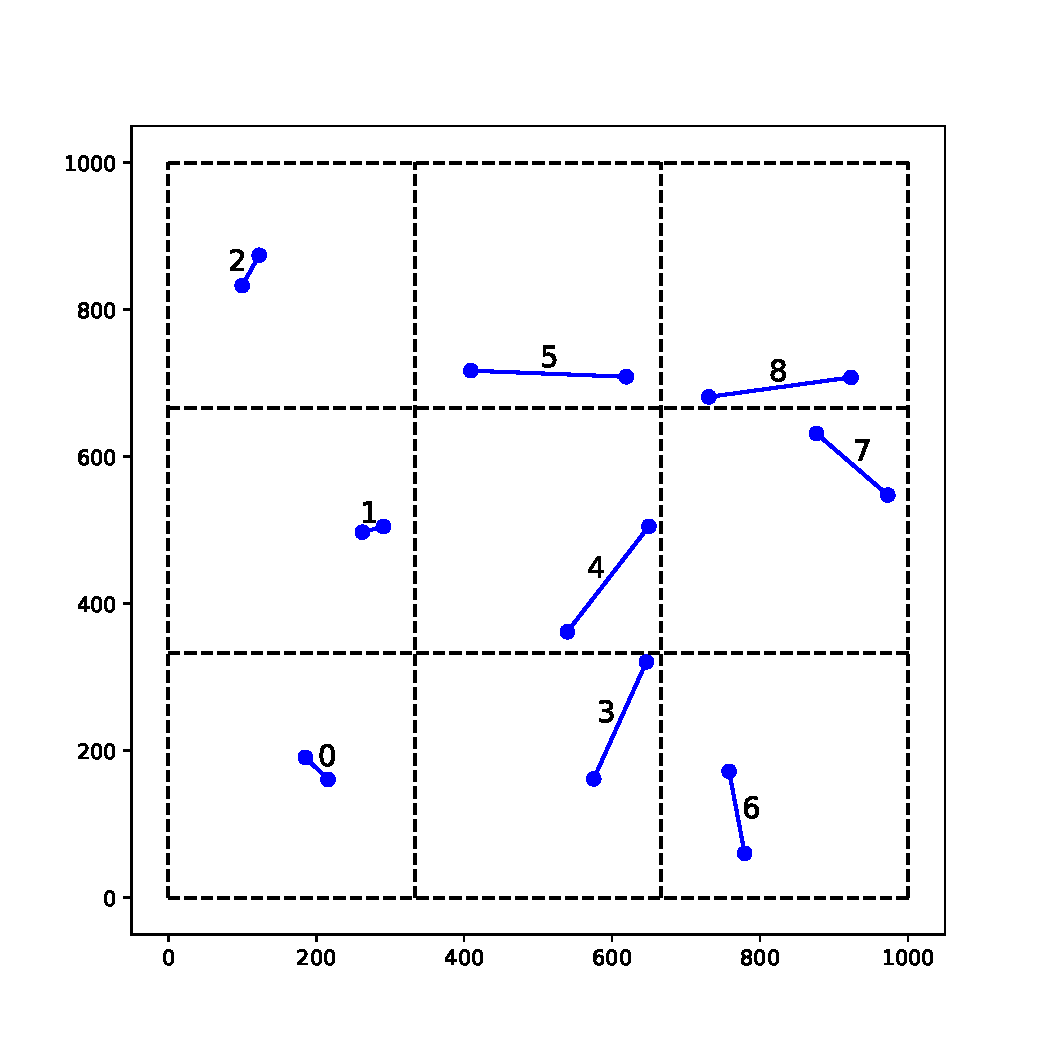
\includegraphics[width=\textwidth]{figs/box_example.pdf}
      \end{figure}
    \end{column}
    \begin{column}{0.65\textwidth}
      \begin{figure}
        \onslide<2>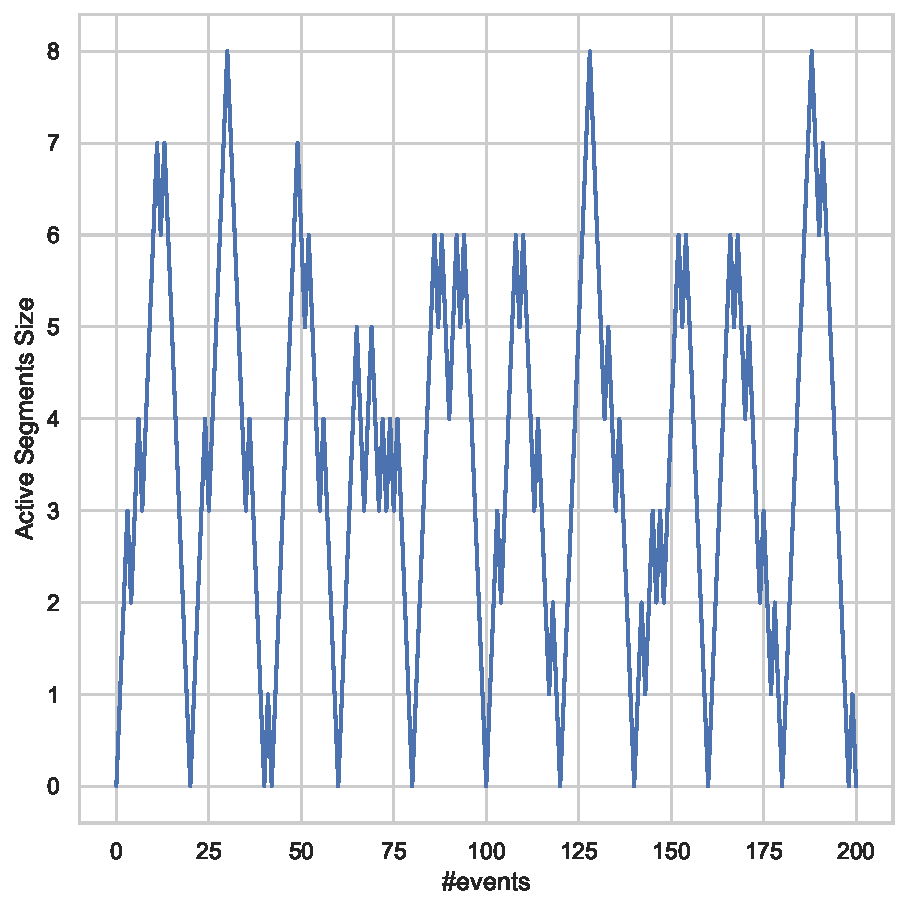
\includegraphics[width=0.8\textwidth]{figs/ativos/small_detection_segments_size_100.pdf}
      \end{figure}
    \end{column}
  \end{columns}
\end{frame}

\begin{frame}{Exemplos Sem Interseção - Segmentos Pequenos}
  % Two columns
     \begin{figure}
        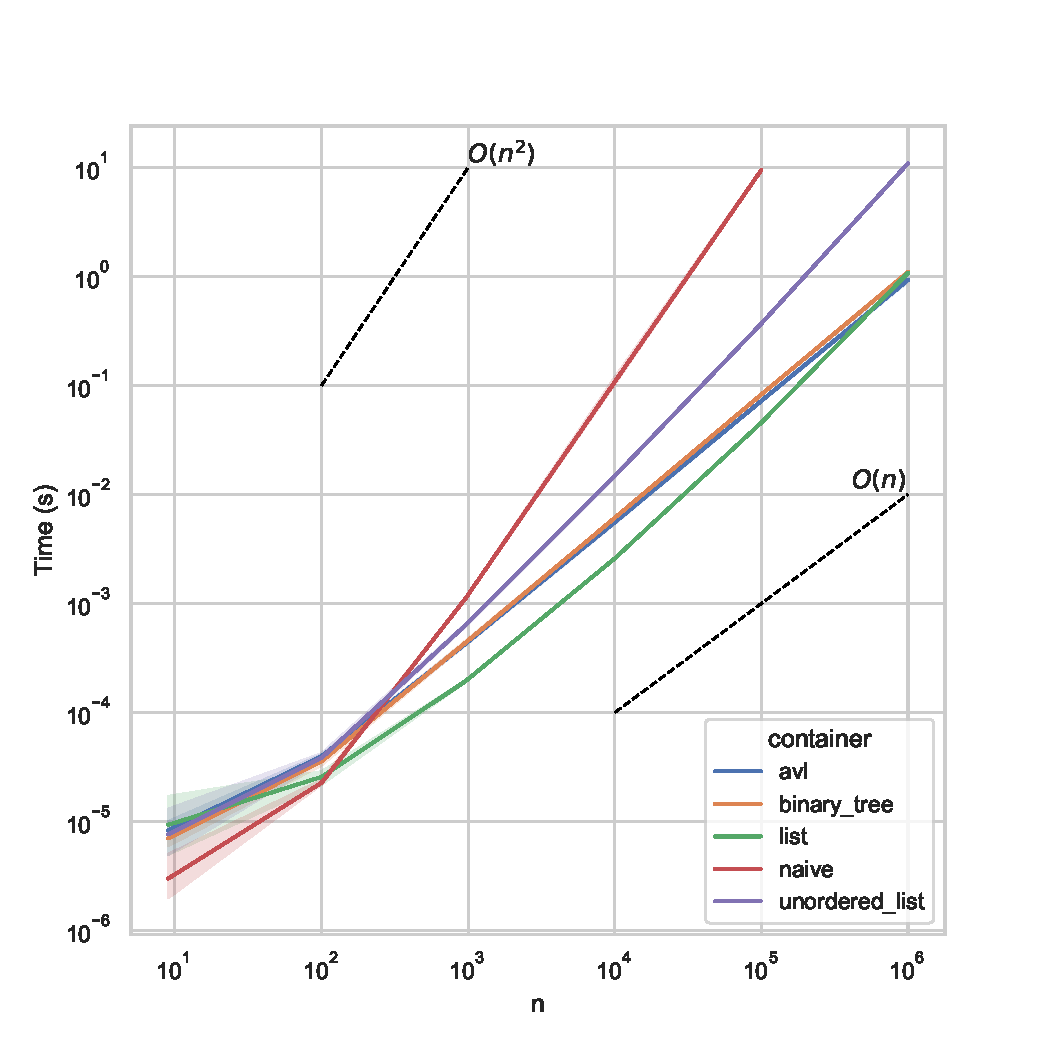
\includegraphics[width=0.5\textwidth]{figs/tempos/plot_small_detection_time.pdf}
      \end{figure}
\end{frame}


\begin{frame}{Algoritmo de Bentley-Ottmann - Listar}
  % Falar sobre algoritmo
  \begin{columns}
      \begin{column}{0.5\textwidth}
        \begin{itemize}
          \item Complexidade $O(n \log n + k \log n )$ 
          \item Lista de eventos varia durante as iterações
          \begin{itemize}
            \item Lista Decrescente
            \item \textbf{Heap-Mínimo}
          \end{itemize}
        \end{itemize}
      \end{column}
      \begin{column}{0.5\textwidth}
      \begin{figure}
        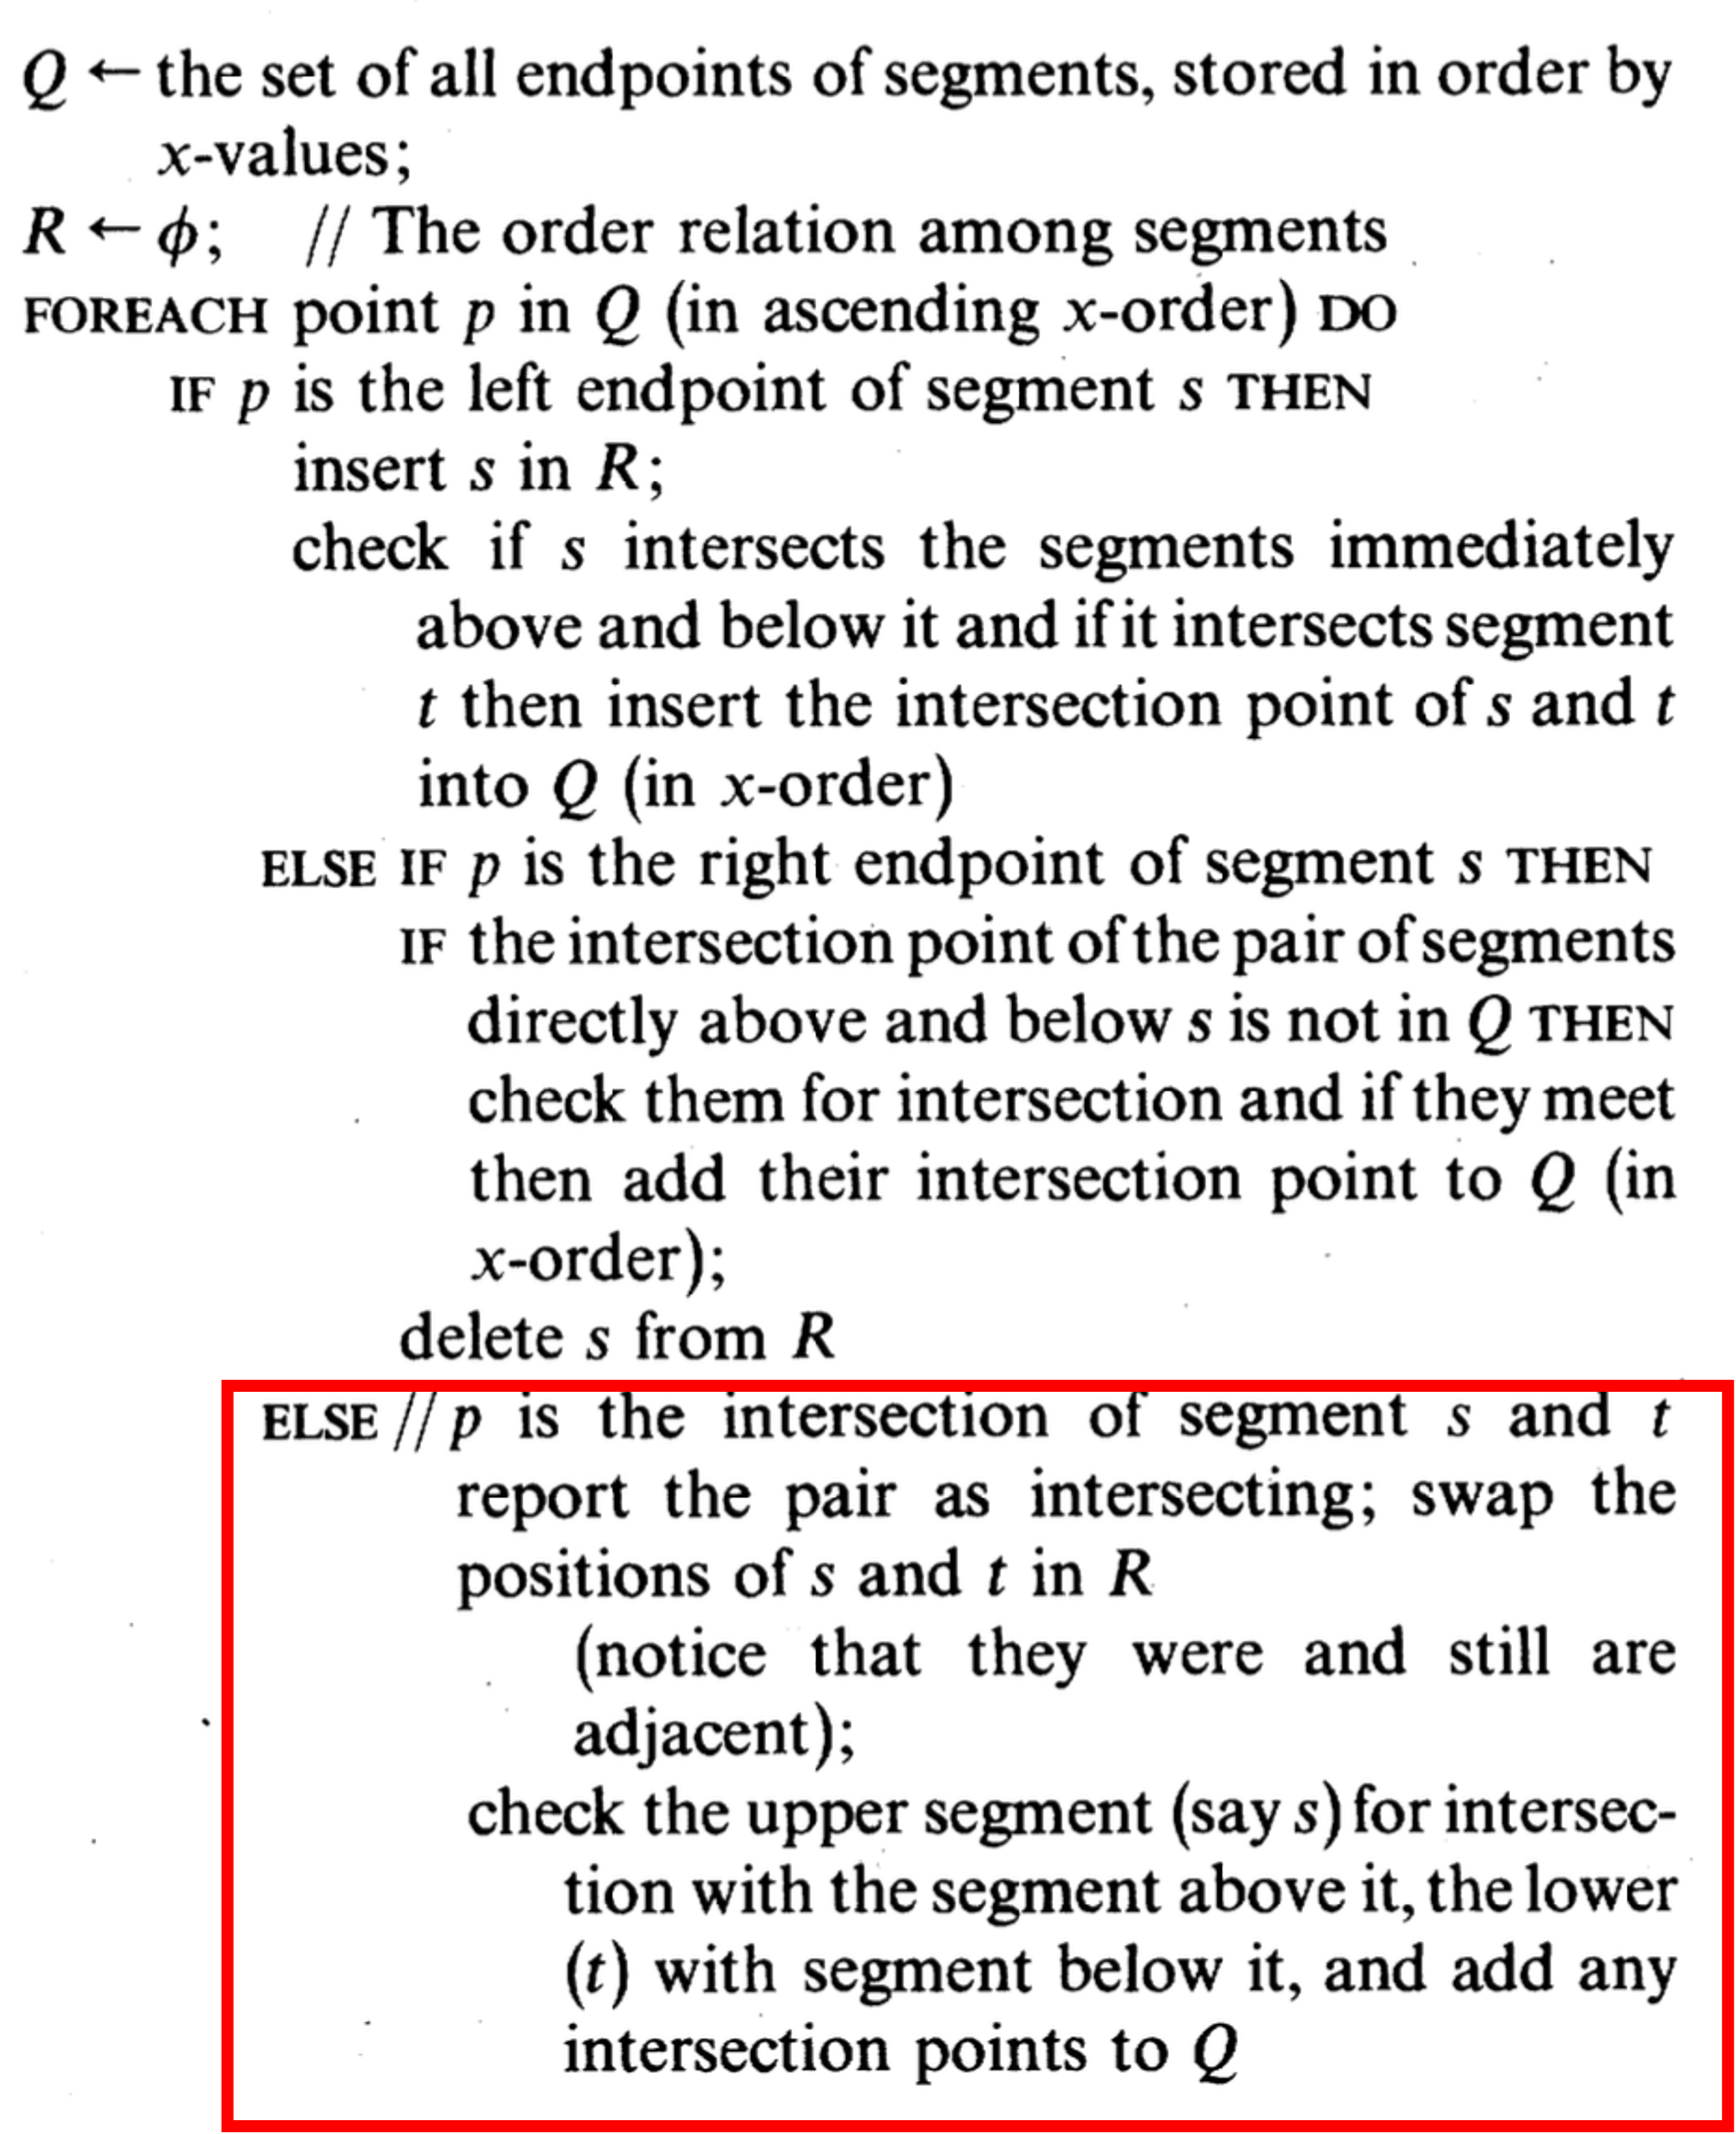
\includegraphics[width=0.9\textwidth]{figs/bentley.png}
        \caption{Força Bruta}
      \end{figure}
      \end{column}
  \end{columns}
\end{frame}

\begin{frame}{Comparação dos segmentos}
  % Falar sobre algoritmo
  \begin{columns}
      \begin{column}{0.5\textwidth}
      \begin{figure}
          
\definecolor{green}{RGB}{0,128,0}
  \begin{tikzpicture}
    % Define the points
    \coordinate (A) at (1, 1); 
    \coordinate (B) at (7,4 );
    \coordinate (C) at (2, 3); 
    \coordinate (D) at (6,1 );
    \coordinate (E) at (4.5, 1.5); 
    \coordinate (F) at (7, 1.5);

    \coordinate(C1) at (2, 0);
    \coordinate(I) at (3.5, 2.25);
    \coordinate(I1) at (3.5, 0);
    \coordinate(E1) at (4.5, 0);
    \coordinate(E2) at (4.5, 3.5); 

    \coordinate(R1) at (2.75, 0);
    \coordinate(R2) at (2.75, 3.5); 
    
    \draw[thick, blue] (A) -- (B);
    \draw[thick, blue] (C) -- (D);
    \draw[thick, blue] (E) -- (F);
    % Draw the points
    \foreach \point in {A,B,C,D,E,F}
      \fill (\point) circle (2pt);

    % \foreach \point in {A,B,C,D,E,F, I}
    %   \node[above right] at (\point) {\point};

    \onslide<2>{
        \draw[dashed, black] (C) -- (C1);
        \draw[dashed, black] (E) -- (E1);
    }
        
    \onslide<2-3>\draw[dashed, black] (I) -- (I1);

    \onslide<3-> \fill[red] (I) circle (2pt);
    \onslide<4> {
        \draw[dashed, black] (R1) -- (R2);
    }


    % \node[above right] at (B) {B};
    % \node[above right] at (C) {C};
    % \node[above right] at (D) {D};
    % \node[above right] at (E) {E};
    % \node[above right] at (F) {F};
    % \node[above right] at (G) {G};
    % \node[above right] at (H) {H};

    
    % Draw the convex hull
    
    

  \end{tikzpicture}

      \end{figure}
      \end{column}
      \begin{column}{0.5\textwidth}
        % Adicionar Figura
        \begin{figure}
        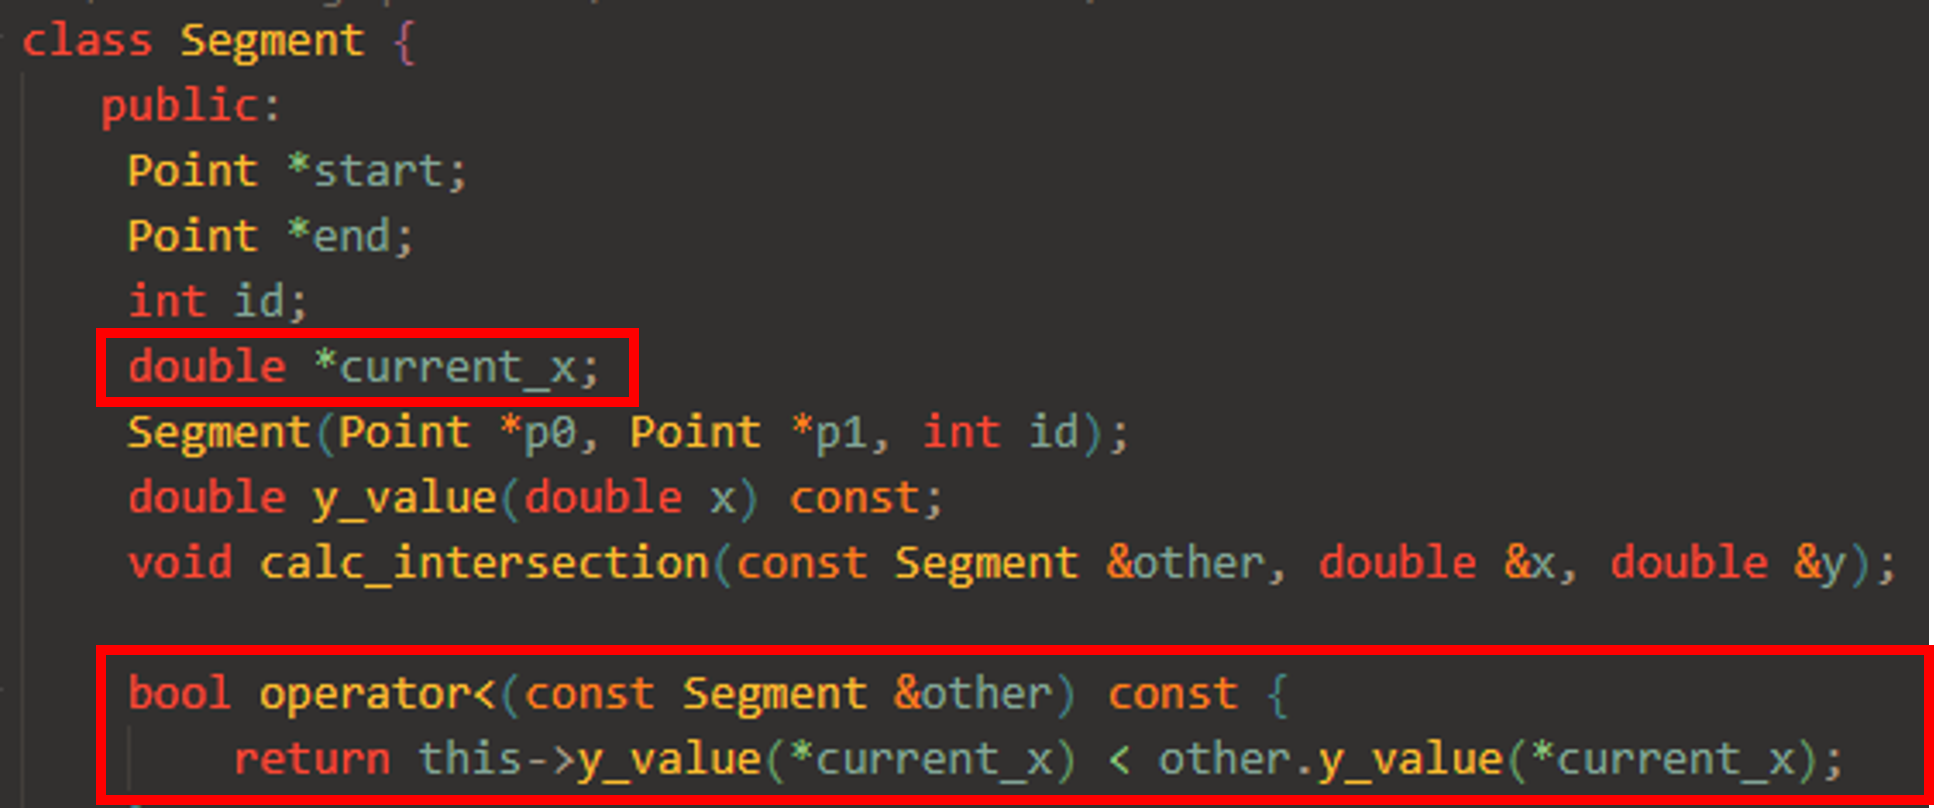
\includegraphics[width=\textwidth]{figs/segment.png}
        \end{figure}
      \end{column}
  \end{columns}
\end{frame}

\begin{frame}{Segmentos Aleatórios}
  \begin{columns}
      \begin{column}{0.5\textwidth}
        \begin{itemize}
          \item Ponto sorteado em $[0, 1] \times [0, 1]$
          \item Ângulo sorteado em $[-\pi, \pi]$
          \item Tamanho Distribuição Normal
        \end{itemize}
      \end{column}
      \begin{column}{0.5\textwidth}
      \begin{figure}
        \begin{tikzpicture}

            % Define the coordinates and angle
            \def\xa{1}
            \def\ya{2}
            \def\thetavala{45}
            \def\lengthval{5}

            % Calculate the second point coordinates
            \pgfmathsetmacro\xb{\xa + \lengthval*cos(\thetavala)}
            \pgfmathsetmacro\yb{\ya + \lengthval*sin(\thetavala)}
            \draw[thick] (\xa, \ya) -- (\xb, \yb);
            \draw[dashed] (\xa, \ya) -- (1.5, \ya);
            \node at (\xa, \ya) [left] {$(x_0, y_0)$};
            \draw[->] (\xa, \ya) +(\thetavala:0.5cm) arc [start angle=\thetavala, end angle=0, radius=0.5cm];
            \node at (\xa, \ya) [right, xshift=0.5cm, yshift=0.2cm] {$\mathbf{\theta_0}$};

            \def\xc{0}
            \def\yc{5}
            \def\thetavalb{330}
            \pgfmathsetmacro\xd{\xc + \lengthval*cos(\thetavalb)}
            \pgfmathsetmacro\yd{\yc + \lengthval*sin(\thetavalb)}
            \draw[thick] (\xc, \yc) -- (\xd, \yd);
            \draw[dashed] (\xc, \yc) -- (0.5, \yc);
            \node at (\xc, \yc) [left] {$(x_1, y_1)$};
            \draw[->] (\xc, \yc) +(\thetavalb:0.5cm) arc [start angle=\thetavalb, end angle=359, radius=0.5cm];
            \node at (\xc, \yc) [right, xshift=0.5cm, yshift=0.2cm] {$\mathbf{\theta_1}$};

        \end{tikzpicture}
        \end{figure}
      \end{column}
  \end{columns}
\end{frame}

\foreach \n in {10, 100} {
\begin{frame}{Exemplos Segmentos Aleatórios - N = \n}
  % Two columns
  \begin{columns}
    \begin{column}{0.5\textwidth}
      \begin{figure}
        \includegraphics[width=\textwidth]{figs/exemplos/random_example_0.1_\n_segments.pdf}
      \end{figure}
    \end{column}
    \begin{column}{0.5\textwidth}
      \begin{figure}
        \includegraphics[width=\textwidth]{figs/exemplos/random_example_0.6_\n_segments.pdf}
      \end{figure}
    \end{column}
  \end{columns}
\end{frame}

\begin{frame}{Exemplos Segmentos Aleatórios - N = \n}
  % Two columns
  \begin{columns}
    \begin{column}{0.5\textwidth}
      \begin{figure}
        \includegraphics[width=\textwidth]{figs/exemplos/random_example_0.1_\n_interserctions.pdf}
      \end{figure}
    \end{column}
    \begin{column}{0.5\textwidth}
      \begin{figure}
        \includegraphics[width=\textwidth]{figs/exemplos/random_example_0.6_\n_interserctions.pdf}
      \end{figure}
    \end{column}
  \end{columns}
\end{frame}
}

\begin{frame}{Comparação com força bruta}
      \begin{figure}
        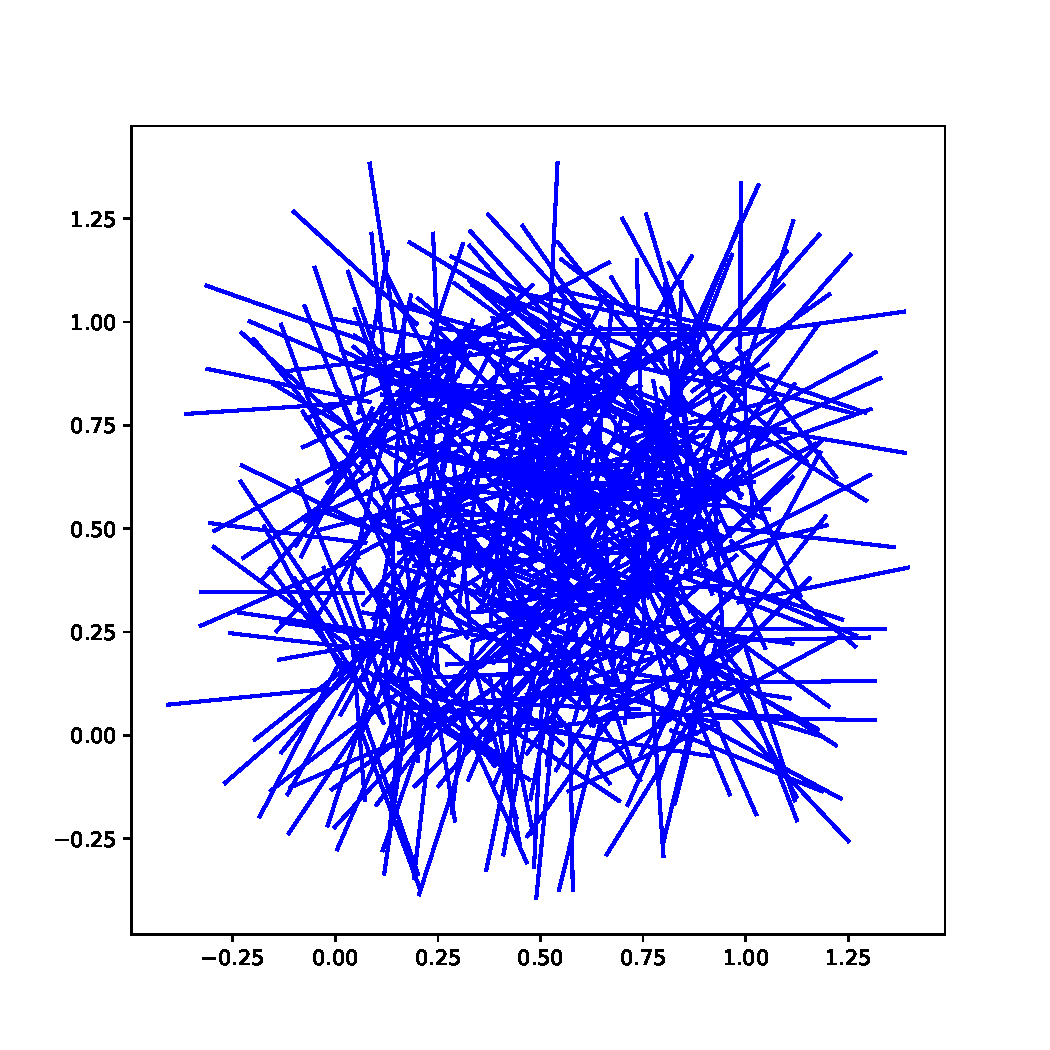
\includegraphics[width=0.6\textwidth]{figs/exemplos/base_segments.pdf}
      \end{figure}
\end{frame}


\begin{frame}{Comparação com força bruta}

  Ordenar as interseções do algoritmo de Bentley-Ottmann e comparar com as interseções do algoritmo de força bruta.

   \begin{columns}
    \begin{column}{0.5\textwidth}
      \begin{figure}
        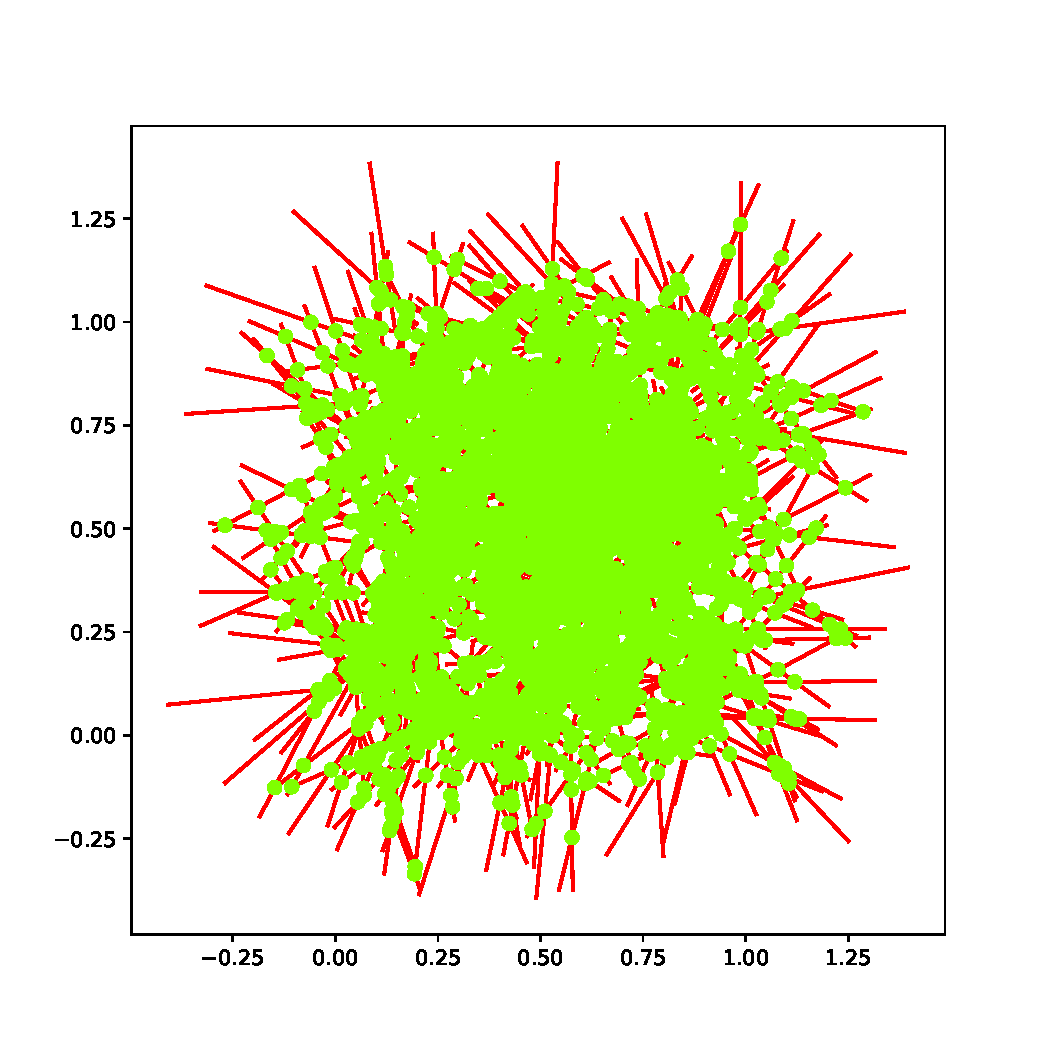
\includegraphics[width=\textwidth]{figs/exemplos/base_naive.pdf}
        \caption{Força Bruta}
      \end{figure}
    \end{column}
    \begin{column}{0.5\textwidth}
      \begin{figure}
        \centering
        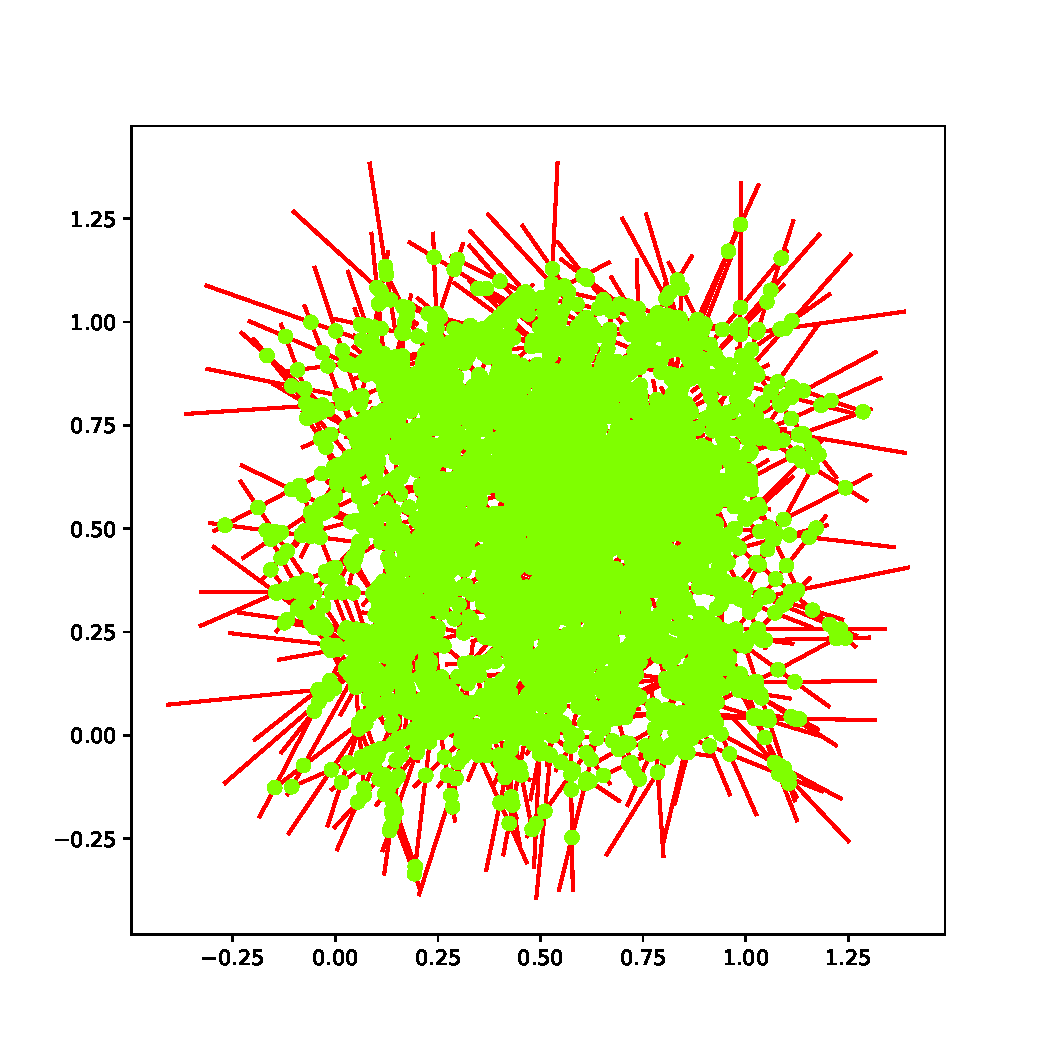
\includegraphics[width=\textwidth]{figs/exemplos/base_avl.pdf}
        \caption{Avl}
      \end{figure}
    \end{column}
  \end{columns}
\end{frame}

\begin{frame}{Segmentos Ativos}

   \begin{columns}
    \begin{column}{0.5\textwidth}
      \begin{figure}
        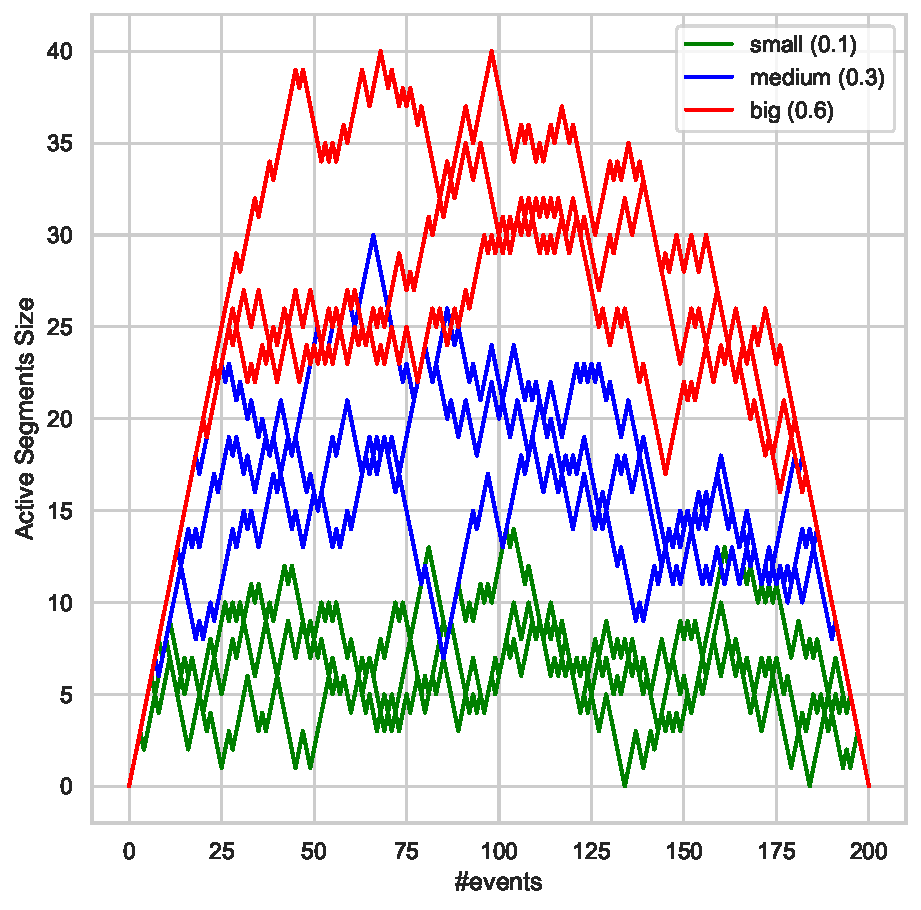
\includegraphics[width=\textwidth]{figs/ativos/active_segments_size_100.pdf}
        \caption{N = 100}
      \end{figure}
    \end{column}
    \begin{column}{0.5\textwidth}
      \begin{figure}
        \centering
        \onslide<2>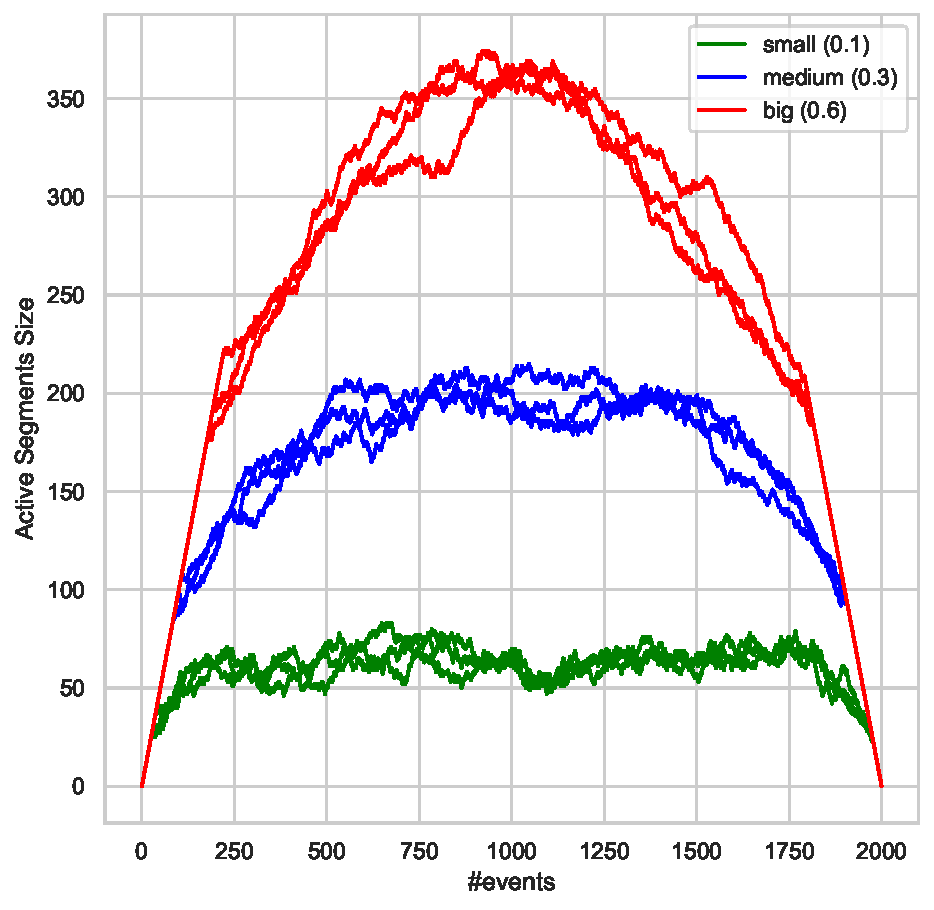
\includegraphics[width=\textwidth]{figs/ativos/active_segments_size_1000.pdf}
        \caption{N = 1000 }
      \end{figure}
    \end{column}
  \end{columns}
 

\end{frame}

\begin{frame}{Segmentos Ativos - Pequenos}
      \begin{figure}
        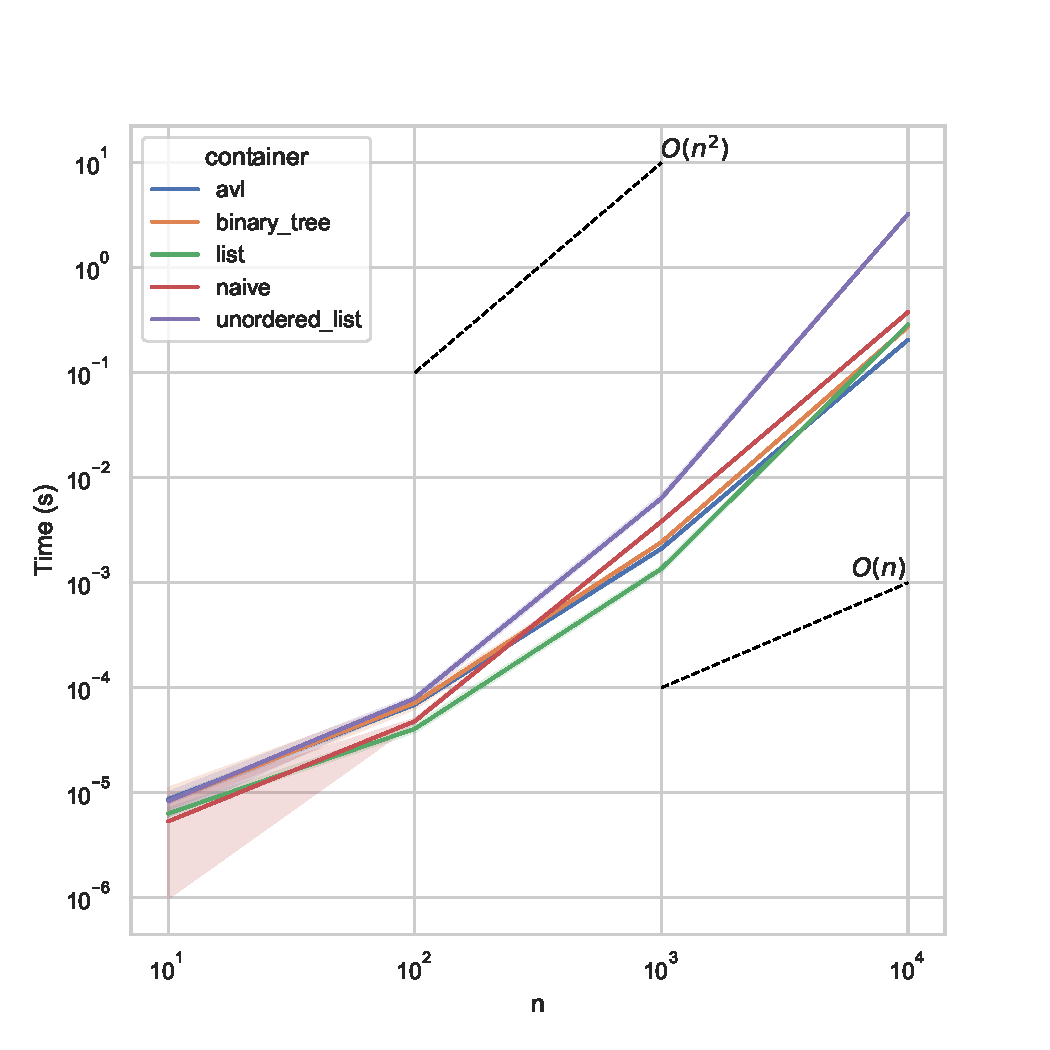
\includegraphics[width=0.5\textwidth]{figs/tempos/plot_random_small_time.pdf}
      \end{figure}
\end{frame}

\begin{frame}{Segmentos Ativos - Médios}
      \begin{figure}
        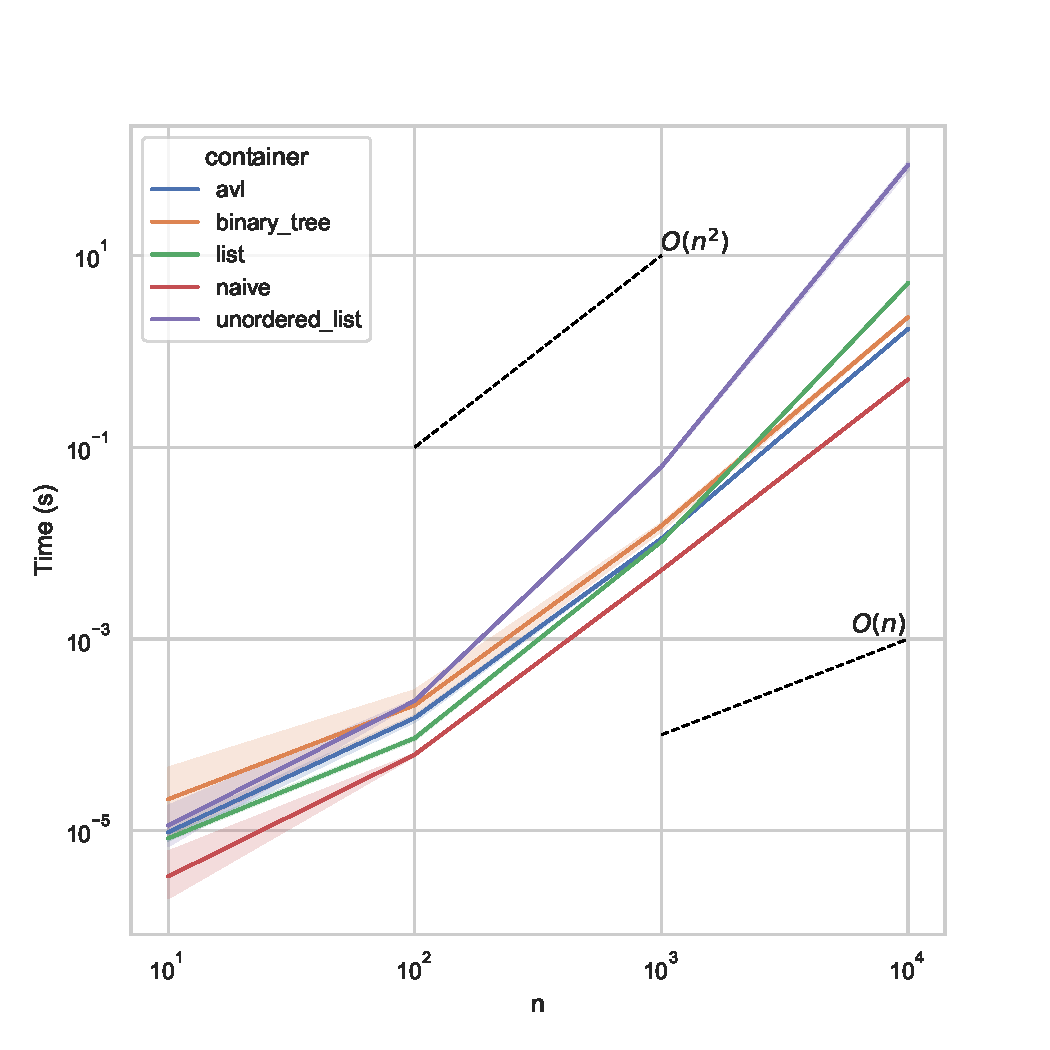
\includegraphics[width=0.5\textwidth]{figs/tempos/plot_random_medium_time.pdf}
      \end{figure}
\end{frame}

\begin{frame}{Segmentos Ativos - Grandes}
      \begin{figure}
        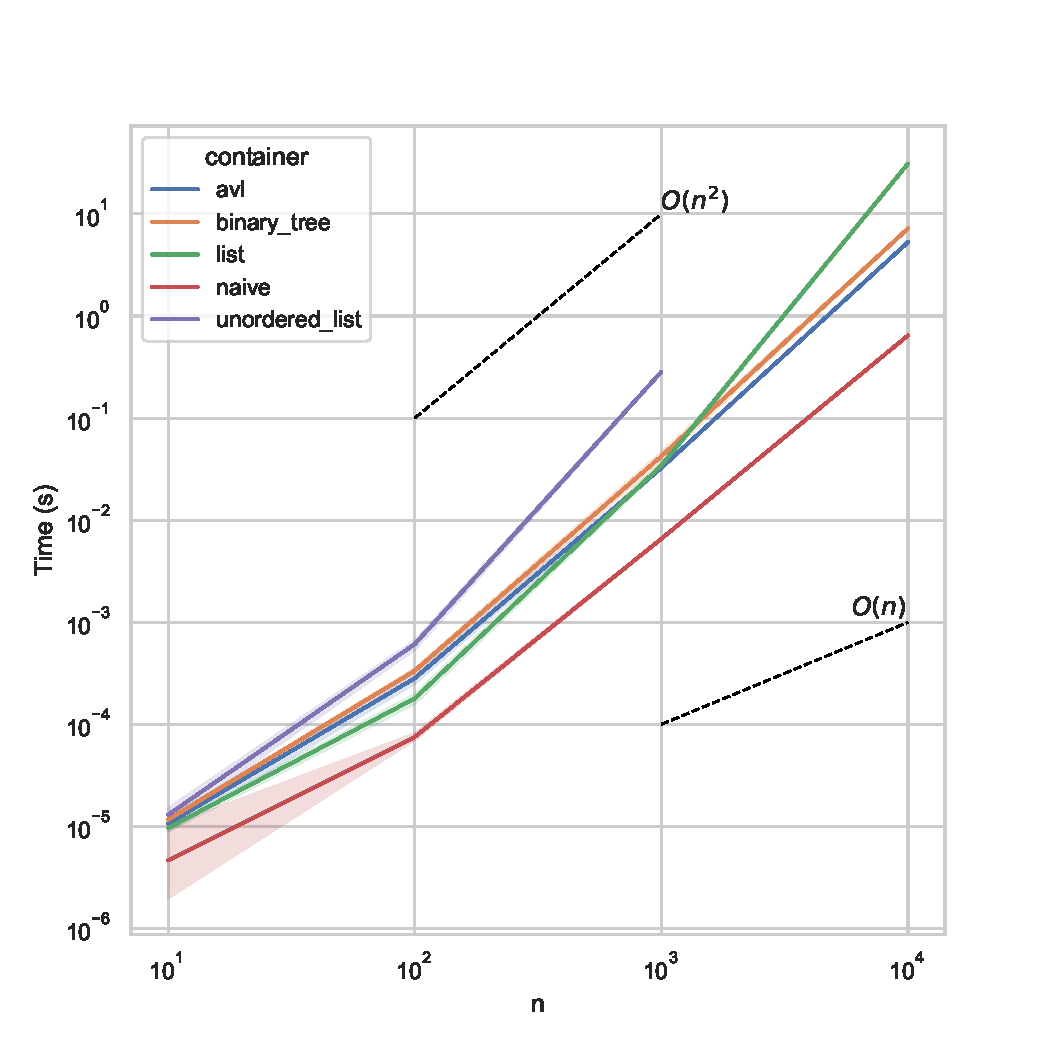
\includegraphics[width=0.5\textwidth]{figs/tempos/plot_random_big_time.pdf}
      \end{figure}
\end{frame}

\begin{frame}{Número de interseções}
  \begin{figure}
    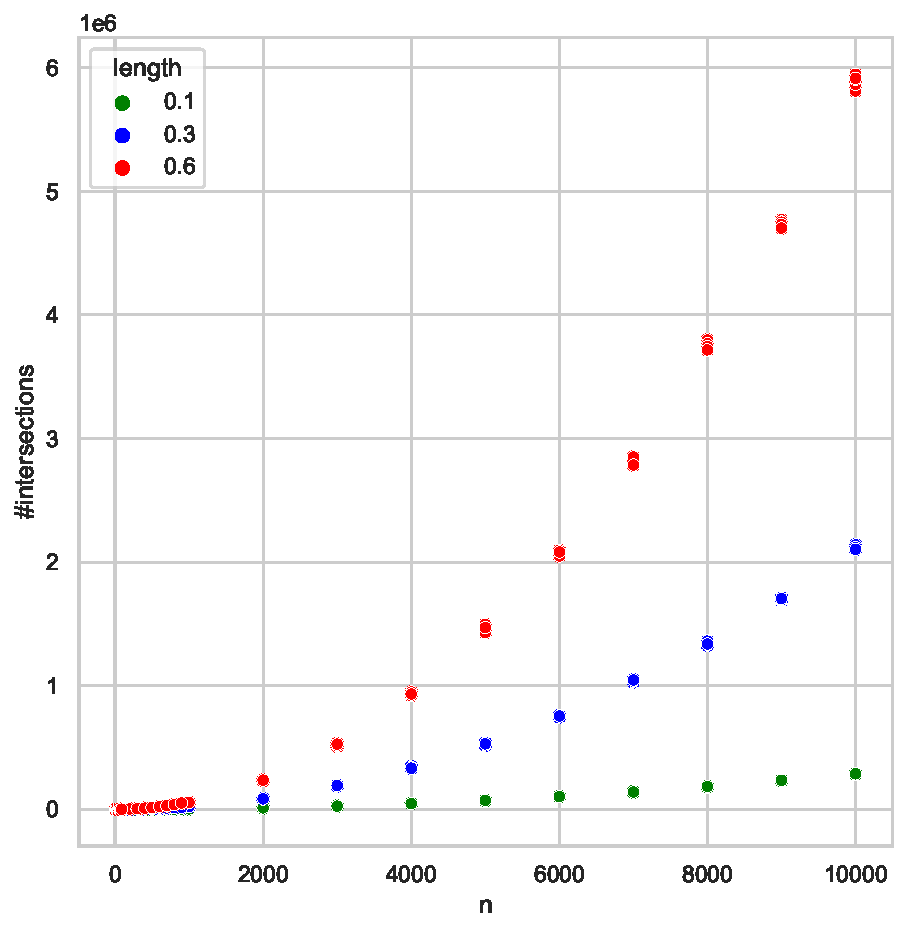
\includegraphics[width=0.5\textwidth]{figs/exemplos/n_intersections.pdf}
  \end{figure}
\end{frame}

\begin{frame}{Número de interseções}
  \begin{figure}
    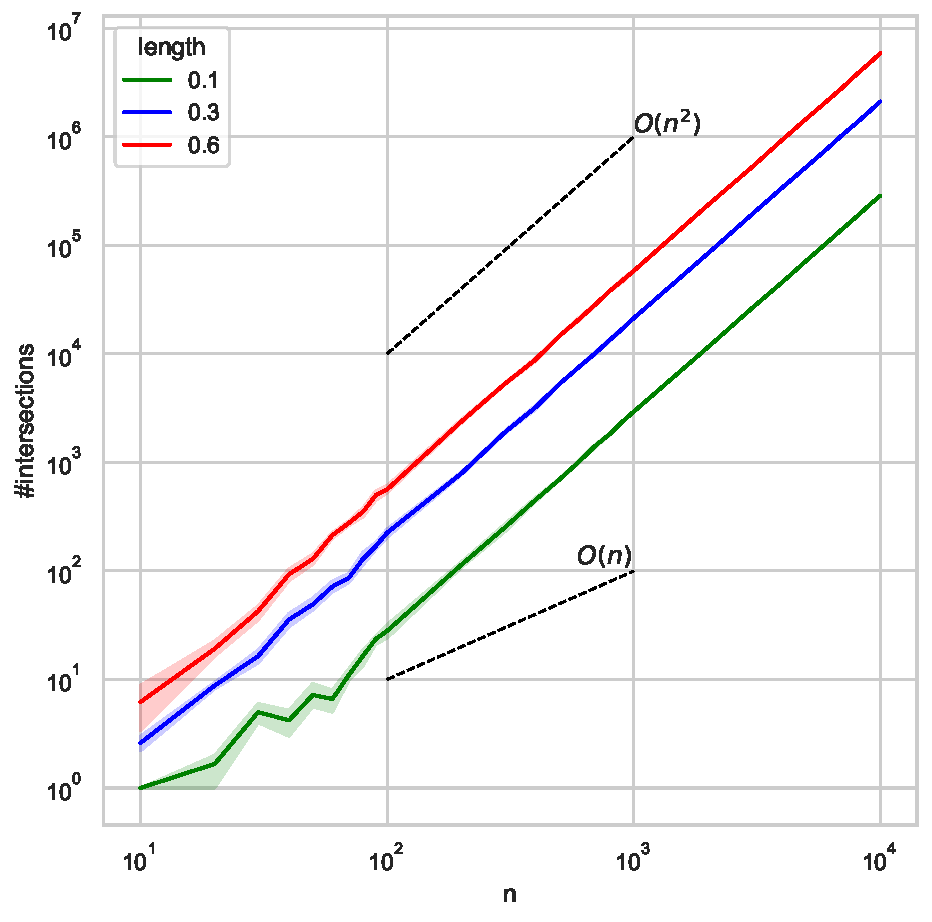
\includegraphics[width=0.5\textwidth]{figs/exemplos/n_intersections_log.pdf}
  \end{figure}
\end{frame}

\begin{frame}{ Eventos: Heap x Lista}

   \begin{columns}
    \begin{column}{0.4\textwidth}
      \begin{figure}
        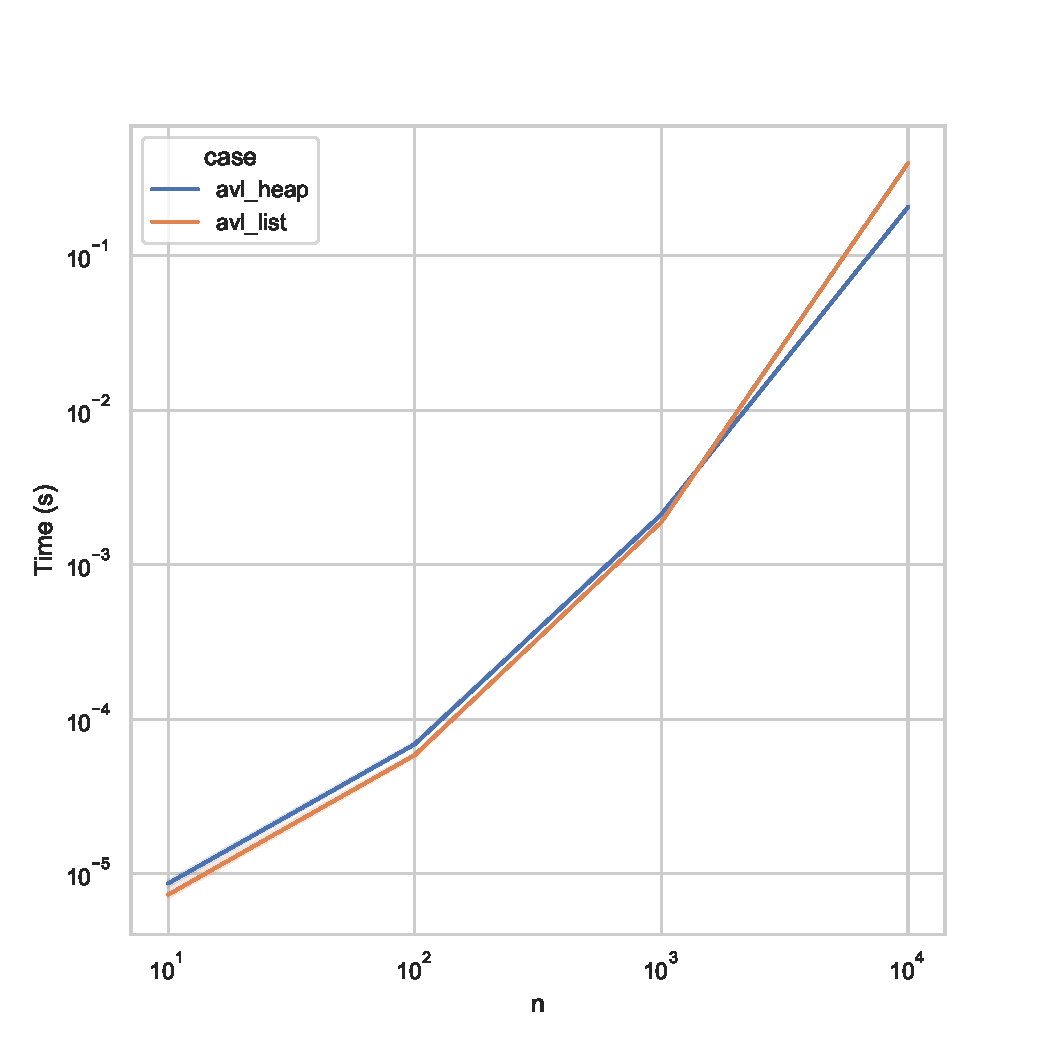
\includegraphics[width=\textwidth]{figs/tempos/heap_x_list_small.pdf}
        \caption{Segmentos Pequenos}
      \end{figure}
    \end{column}
    \begin{column}{0.4\textwidth}
      \begin{figure}
        \centering
        \onslide<2>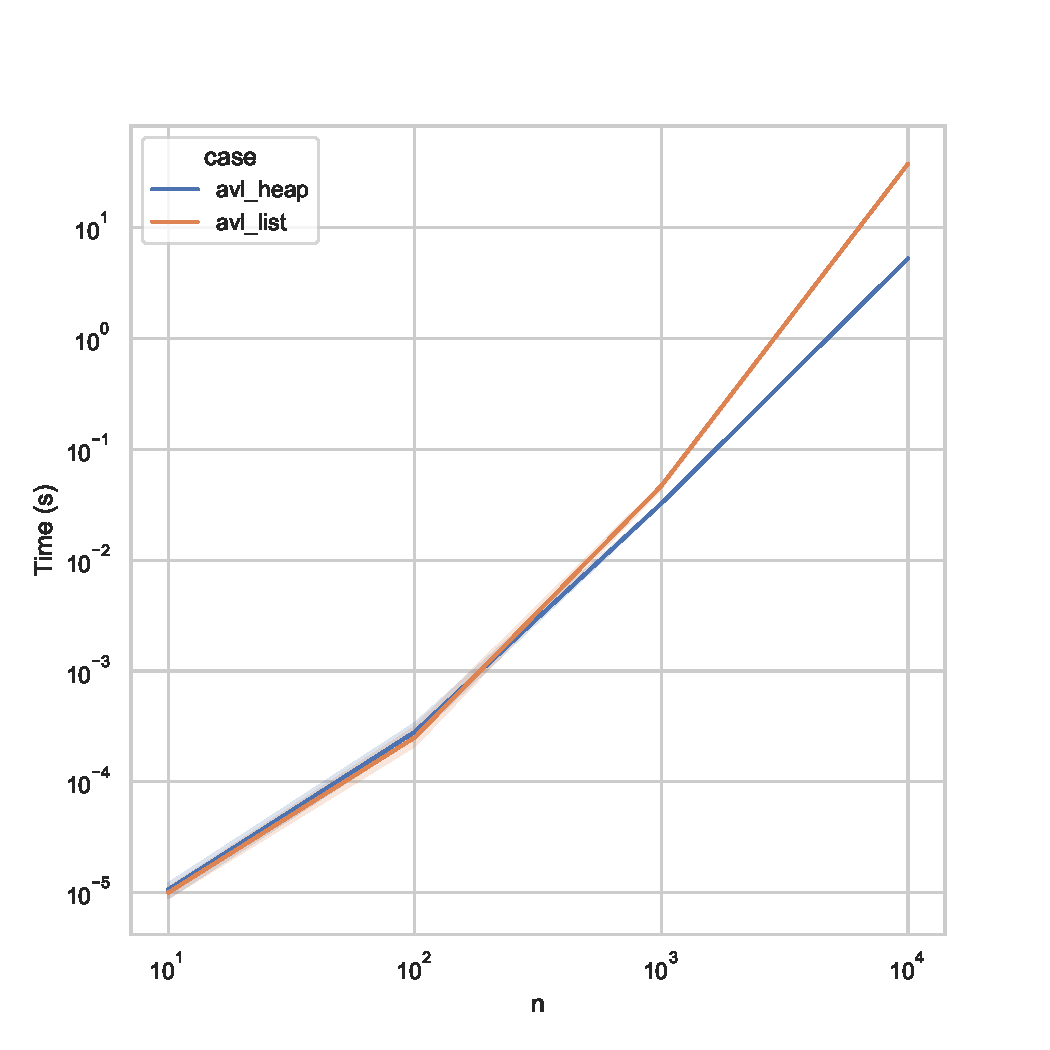
\includegraphics[width=\textwidth]{figs/tempos/heap_x_list_big.pdf}
        \caption{Segmentos Grandes}
      \end{figure}
    \end{column}
  \end{columns}
 

\end{frame}


\begin{frame}{Exemplo Grid}
  % Two columns
  \begin{columns}
    \begin{column}{0.35\textwidth}
    \begin{center}
      \begin{figure}
        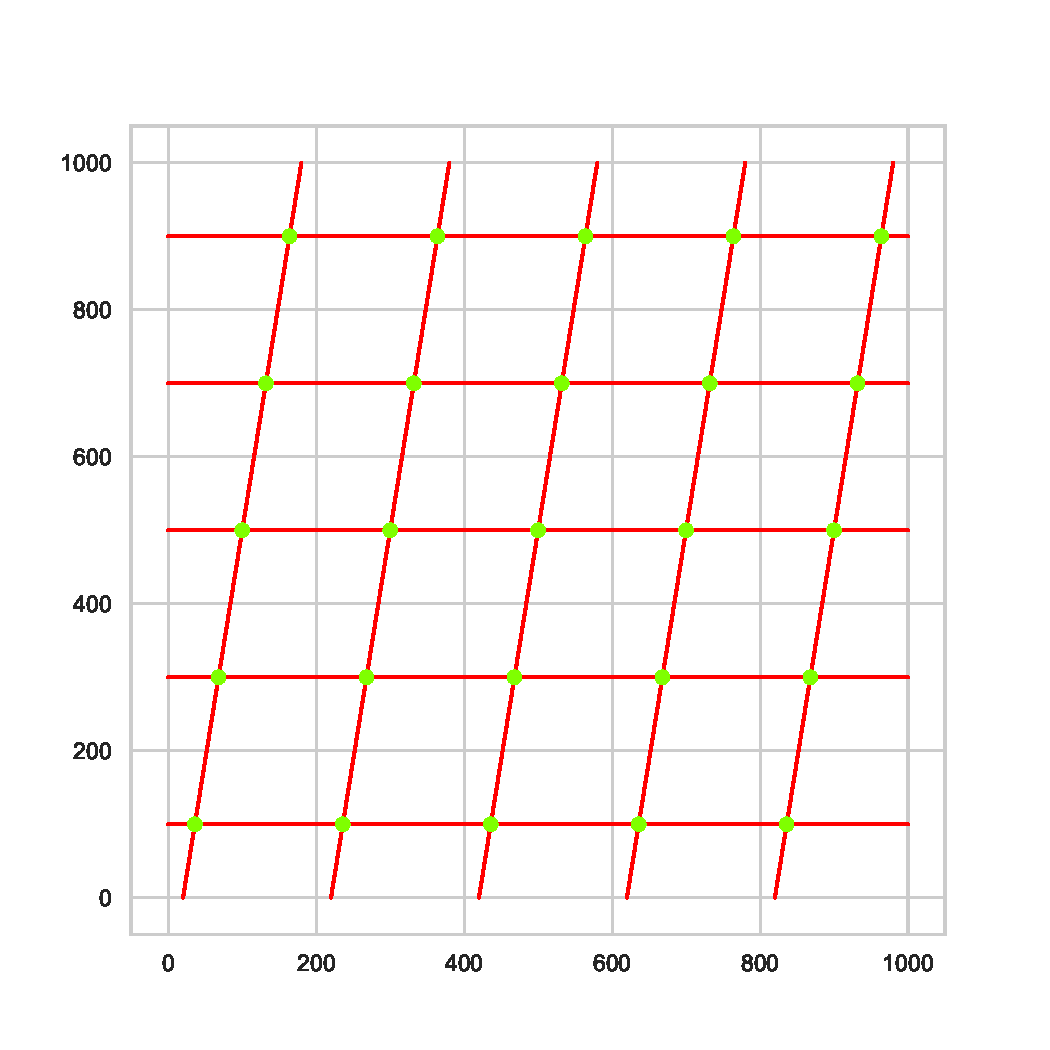
\includegraphics[width=\textwidth]{figs/exemplos/grid_example_10_interserctions.pdf}
      \end{figure}
      $k = n^2/4$
    \end{center}
    \end{column}
    \begin{column}{0.65\textwidth}
      \begin{figure}
        \onslide<2>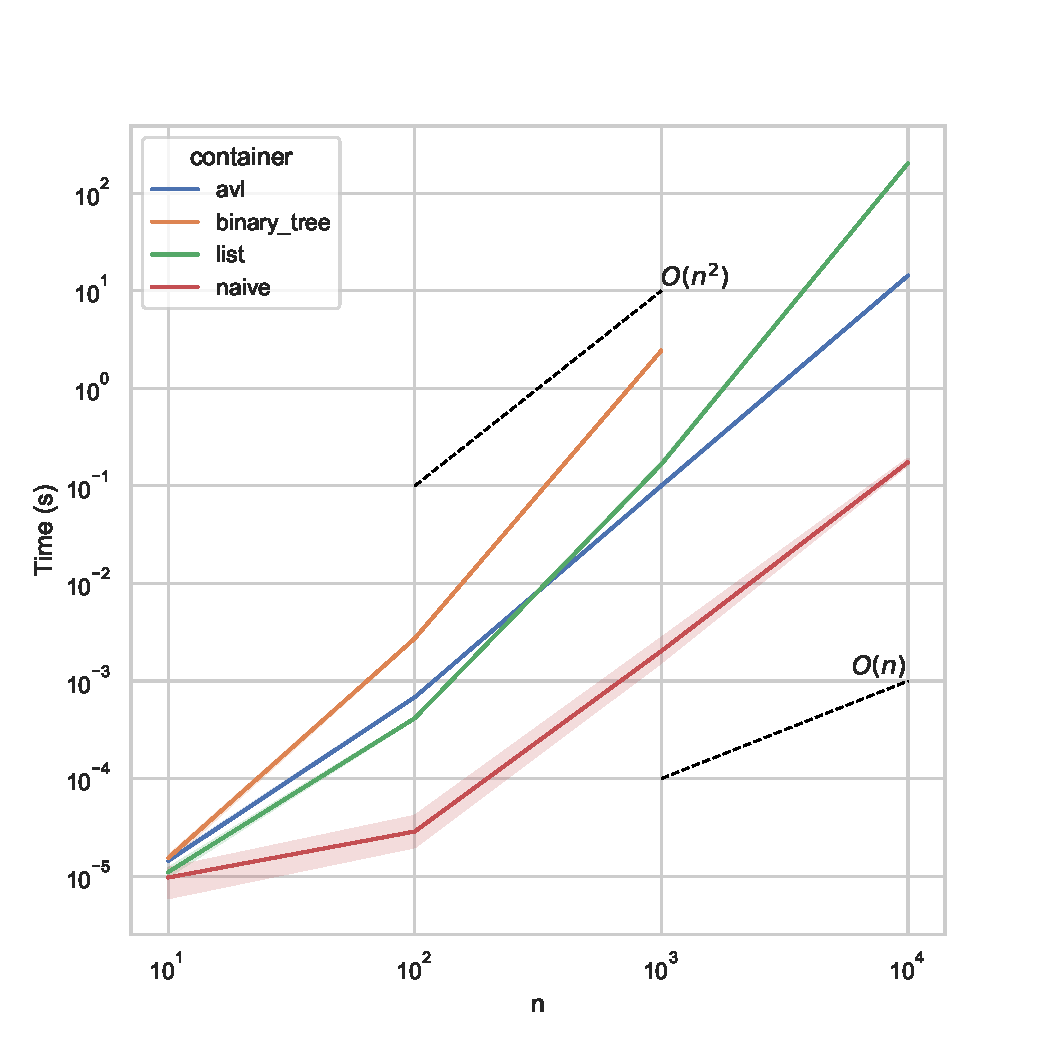
\includegraphics[width=0.8\textwidth]{figs/tempos/plot_grid_time.pdf}
      \end{figure}
    \end{column}
  \end{columns}
\end{frame}

\begin{frame}{Conclusões}

  \begin{itemize}
    \item O algoritmo de Bentley-Ottmann funciona O(n log n) na detecção
    \item O algoritmo de Bentley-Ottmann pode ir pior que a força bruta em problemas com muitas interseções
    \item O uso de estrutura de dados de árvore balanceada são necessárias para obter a complexidade ótima.
  \end{itemize}
  
\end{frame}



\end{document}